%=========================================
% 	   Einleitung     		 =
%=========================================
\chapter{Einleitung}
\section{Vorstellung des Themas}
Der nachfolgende Beitrag beschäftigt sich mit der Führung von Team mit der Zielsetzung die Performance von Teams zu optimieren.\\\\
Teammanagement hat es zum Ziel, eine Gruppe von Individuen zu einem kohärenten Team zu verschmelzen, das zusammen ein gemeinsames Ziel erreicht. Zum Management von Teams gehören das Erarbeiten der Aufgaben des Teams, das Definieren von Rollen im Team, das Erschaffen von Strukturen sowie das Fördern der Zusammenarbeit von Teammitgliedern als auch die Führung selbst.\\\\
Hinsichtlich der Softwareentwicklung gibt es gewisse Punkte, die ein spezielles Augenmerk einfordern. Aufgrund agiler Methoden, wie zum Beispiel Scrum oder Kanban, ist Flexibilität von besonderer Bedeutung, um adaptiv und damit offen für die ständigen Änderungen zu sein. Auch hat Softwareentwicklung einen sehr hohen Anspruch an die Zusammenarbeit zwischen verschiedenen Rollen, wie zum Beispiel Entwicklern selbst oder Testern, sowohl innerhalb von Teams als auch zwischen verschiedenen Teams. Des Weiteren ist durch die ständige Änderung und Weiterentwicklung der Grundlagen der Softwareentwicklung sowohl die Pflege als auch die Förderung der Fähigkeiten und des Wissens der Teammitgliedern von großer Bedeutung.
\section{Motivation und Zielsetzung}
Relevant ist es bei diesem Thema auch, dass häufige Irrglauben aus der Welt geschaffen werden. So korreliert die Größe eines Teams nicht durchwegs mit seiner Produktivität. Auch ist die Rolle des Führungsstils üblicherweise überbewertet. Die negativen Auswirkungen von Harmonie auf die Fehlerkultur und Faulenzer werden meistens nicht berücksichtigt oder das Misstrauen, welches diese in Schach hält, mitsamt seinen Nachteilen gebilligt.\\\\
Die Folgen von gutem Teammanagement und der damit folgende Wert für ein Unternehmen sind erhöhte Effizienz und Effektivität von Teams. Dies geschieht durch eine verbesserte Kommunikation, größere Motivation und Arbeitsmoral durch ein positives Umfeld. Auch wird durch stetiges Einbinden und Unterstützen der Teammitglieder deren Fähigkeiten geschult und etwaige Defizite behoben und dadurch eine Zusammengehörigkeit geschaffen, die die Wahrscheinlichkeit des Verbleibs der Mitarbeiter erhöht.\\\\
Daher ist die Zielsetzung dieser Arbeit, die Faktoren herauszuarbeiten, welche, nach Hackman, für das erfolgreiche Führen und Managen von Teams entscheidend sind.

\chapter{Grundlagen des Teammanagements}
%*****************************************

\section{Definition von Teams }
Ein wichtige, aber nicht offensichtliche Grundlage von dem Verständnis und damit dem Management von Teams ist die Frage, was ein Team überhaupt ist. Hierbei lässt sich grundlegend zwischen Arbeitsgruppen und Teams differenzieren. Während beide gerne als gleichwertig gesehen werden, zeichnen sich in der Praxis starke Kontraste ab.\\\\
Der Unterschied kann damit zusammengefasst werden, dass die Mitglieder einer Arbeitsgruppe eine starke Individualität aufweisen, während einem Team ein Kollektiv zu Grunde legt. Dieser Unterschied zieht sich durch alle relevanten Merkmale von Gruppen. So sollte die Komposition eines Teams ein gutes Zusammenspiel von Fähigkeiten und Persönlichkeiten sicherstellen, um eine gemeinsame Aufgabe zu erledigen, während die Mitglieder in einer Arbeitsgruppe üblicherweise eigene Aufgaben haben und diese eigenständig erledigen. Auch ist die Frage, wie Aufgaben bewältigt werden in Teams eine Frage des Konsenses zwischen den Mitgliedern und einer potenziellen Führungskraft, während dies in Arbeitsgruppen entweder individuell entschieden oder von einer Führungskraft vorherbestimmt wird. Auch ist dieser Unterschied hinsichtlich von Pflichten und Verantwortung gegeben, so sind diese im Team stets zu einem gewissen Grad auf die Mitglieder aufgeteilt im Gegensatz zu Arbeitsgruppen, in denen diese entweder der Führungskraft obliegen oder den einzelnen Mitgliedern selbst.

\section{Theoretische Grundlagen }
Um eine gute Performance von Teams zu gewährleisten sind laut Hackman fünf Prinzipien von besonderer Bedeutung wie man in Abbildung \ref{fig:Hackmann} sehen kann.
%\begin{itemize}
%	\item Real Team
%	\item Compelling Direction
%	\item Enabling Structure
%	\item Supportive Organizational Structure
%	\item Expert Coaching
%\end{itemize}

\begin{figure}[bth]
  \centering
  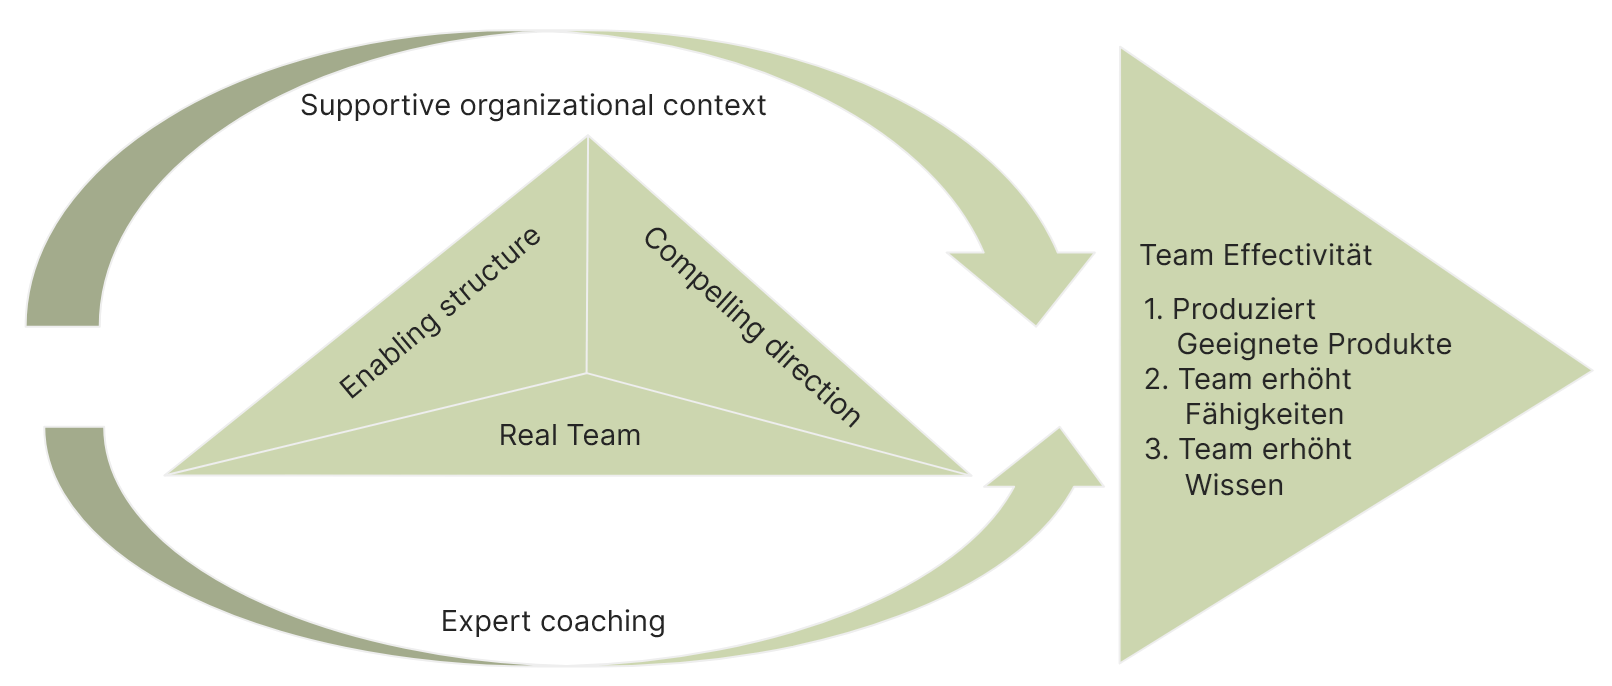
\includegraphics[width=0.7\textwidth]{Examples/Hackman.png}
  \caption{Die fünf Grundlagen für erfolgreiche Team nach Hackmann}
  \label{fig:Hackmann}
\end{figure}


\chapter{Die fünf Grundlagen für erfolgreiche Team nach Hackmann}
\section{Echte Teams}
Das erste Prinzip von Hackman hat er als „Real Team“ betitelt. Hierbei geht es hauptsächlich um die bereits in der Abgrenzung zu Arbeitsgruppen angemerkten inhärenten Kollektivität von Teams, wodurch diese Aufgaben als Einheit erledigen und Ziele gemeinsam erreichen und nicht durch einzelne Mitglieder.
\subsection{Teamaufgaben}
Hinsichtlich Aufgaben bedeutet dies, dass sie sowohl für alle Teammitglieder relevant sein müssen als auch alle an ihrer Lösung mitarbeiten. Daher ist es wichtig, eine für das Team geeignete Aufgabe bereitzustellen. Hierbei ist zu beachten, dass nicht jede Aufgabe für jede Teamgröße oder überhaupt für Teams geeignet ist. So sind Führungs- und Kreativaufgaben üblicherweise eher für Individuen als für Teams geeignet.
\subsection{Klare Zugehörigkeiten}
Um die Leistung sicherzustellen, muss das Team sich sowohl bewusst sein, wer ein Mitglied ist als auch wer kein Mitglied ist. Wichtig ist hier, dass dies keine dynamischen Teams oder das Einbringen teamfremder Experten verbietet, solange diese Umstände allen bewusst sind. Auch sollte jedes Mitglied sich seiner Zugehörigkeit zur aktuellen Teamaufgabe bewusst sein und das Team als Ganzes seiner Bedeutung in der Organisation.
\subsection{Begrenzte Autorität}
Die Autorität innerhalb eines Teams sollte zwar keinesfalls vollkommen einem einzelnen Teammitglied oder einer Führungskraft auferlegt werden, allerdings ist der ideale Grad der Selbstverwaltung von Team zu Team verschieden. Dennoch muss dies allen Mitgliedern bewusst sein. Grob können vier Autoritätsebenen definiert werden, das simple Ausführen der Teamaufgaben, das Überwachen und Managen der Leistung, das Teamdesign sowie die Bedeutung innerhalb der Organisation und die Ausrichtung des Teams.
\subsection{Fortlaufende Stabilität}
Die Zugehörigkeit der Teammitglieder auf Dauer stabil zu halten, erlaubt es dem Team Vertrauen aufzubauen und eine effiziente und effektive Kommunikation zu entwickeln, welche für wichtig für eine gute Performance sind. Des Weiteren erlaubt eine langfristige Zusammenarbeit es den Teammitgliedern, ein tiefes Verständnis ihrer Stärken und Schwächen zu erlangen und dadurch die Aufgaben ideal innerhalb des Teams verteilen und Schwächen auf Dauer beheben zu können.

\section{Beflügelnde Direktive}
Nach Hackman als „Compelling Directive“ bezeichnet besagt dieser Punkt aus, dass ein gutes Management ein Team stets mit Aufgaben versorgt, die ambitioniert, erreichbar und klar definiert sind. Darüber hinaus sind eine eindeutige Richtung sowie die Teilhabe aller Mitglieder von Bedeutung. Die Ziele des Teams sollten stets mit den Zielen der Organisation übereinstimmen und den Teammitgliedern eine Sinnhaftigkeit der Arbeit vermitteln.
\subsection{Ansporn}
Es ist wichtig, die Aufgaben eines Teams so zu setzen, dass jedes Teammitglied von der Aufgabe gefordert wird, damit die Teammitglieder und somit das Team eine intrinsische Motivation zur Lösung der Aufgabe entwickeln. Eine Unterforderung führt in der Regel zu mangelnder Motivation und mangelndem Fokus, was Flüchtigkeitsfehler verursacht. Überforderung hingegen, vor allem auf Dauer, verursacht Frustration, die sich in negativem Verhalten äußern kann.
\subsection{Orientierung}
Die Ziele des Teams müssen wohl definiert sein. Damit wir erlaubt, dass sowohl die Organisation als auch das Team selbst den Fortschritt nachvollziehen kann und dadurch bewusst Erfolge erfahren können, was die Motivation steigert oder Missstände erkennen und diese durch eine frühzeitige Änderung des Zieles oder Umverteilung von Ressourcen beheben kann. Auch wird hierdurch sichergestellt, dass das gesamte Team das gleiche Ziel mit der gleichen Strategie verfolgt.
\subsection{Teilhabe}
Auch ist es bei den Aufgaben und Zielen des Teams für die Motivation wichtig, dass jedes Mitglied zu jedem Zeitpunkt einen Teil zur Lösung der aktuellen Aufgabe beiträgt. Um dies sicherzustellen, sollte Wert daraufgelegt werden, dass die Teilaufgaben entweder den Expertisen der einzelnen Teammitglieder entsprechen oder dazu führen, dass ein Mitglied seine Expertise zu Teilen an andere Mitglieder weitergeben kann. Auch ist hier zu beachten, dass in einem zu großen Team gegebenenfalls nicht die Nötige Auslastung vorhanden ist was dazu führen kann, dass sich einzelne Teammitglieder aus dem Team ausklinken.
\subsection{Balance}
Bei diesen drei Punkten ist nochmal hervorzuheben, dass die Balance von äußerster Bedeutung ist. Der Frust einer zu großen Herausforderung kann ein Team auf Dauer zersetzen, während eine mangelnde Herausforderung die Weiterentwicklung des Teams gefährdet. Ein Mangel an Orientierung hingegen kann ein Team auseinandertreiben, während zu expliziten Anweisungen die Kreativität einschränkt.  Eine mangelnde Teilhabe hingegen kann zur Abschottung von Individuen führen, während eine zu große Teilhabe eine Abhängigkeit vom Individuum erzeugt.

\section{Befähigende Struktur}
Bei der „Enabling Structure” geht es darum, die Strukturen, die dem Miteinander zugrunde legen so zu erschaffen, dass der Teamgeist und die Zusammenarbeit gefördert und nicht behindert werden.
\subsection{Verhaltensregeln}
Verhaltensregeln und Umgangsformen werden benötigt, um ein Zuverlässiges Team zu gestalten. Hierbei ist wichtig diese im Rahmen des Teams zu verhandeln, da die richtigen Verhaltensregeln vollkommen von den einzelnen Teammitgliedern abhängig sind. Dennoch können zwei generelle Punkte angemerkt werden die inhärent für Teamarbeit sind. So sollten die Teammitglieder stets aufmerksam und proaktiv arbeiten und sich den aktuellen Gegebenheiten anpassen zu können. Des Weiteren sollten zumindest die wichtigsten Musts und No-Gos herausgearbeitet werden, um ein sicheres Miteinander zu gewährleisten.
\subsection{Größe}
Bei der Teamgröße ist es für eine gute Performance wichtig das richtige Mittel an Mitgliedern zu finden. Es muss eine ausreichende Diversität an Fähigkeiten vorliegen um die Aufgabe zu bewältigen und dabei alle Teammitglieder auszulasten. Aber dennoch klein genug sein, um effiziente Kommunikation und eine klare Verteilung der Aufgaben zu gewährleisten. Nach Vidmar liegt die ideale Teamgröße, nach einer Selbsteinschätzung von Teams, bei vier oder fünf Mitgliedern \cite{a985d9bd-bc17-3a58-b90d-1cca2b2b7d68}.
\subsection{Komposition}
Bei der Zusammenstellung eines Teams ist darauf zu achten, dass das Team die für die zu erwartenden Aufgaben erforderlichen Fähigkeiten und Wissen aufweist. Auch ist zu beachten, dass das Team eine angemessene Größe hat. Während gewisse Aufgaben eine Mindestgröße benötigt erhöht sich mit steigender Zahl der Mitglieder der organisatorische Aufwand und die Qualität der Kommunikation sinkt.
\subsection{Soziale Fähigkeiten}
Die sozialen Fähigkeiten der Mitglieder sind ein komplexer, aber relevanter Faktor im Management von Teams. Die interpersonellen Fähigkeiten und Charakterzüge von Personen sind nicht immer kompatibel und müssen daher berücksichtigt werden. Hierbei ist ein zu großes Augenmerk auf Harmonie fehl am Platz. Auch ist wichtig anzumerken, dass nicht jede Person für Teamarbeit geeignet ist, dennoch ist es an der Führung zu evaluieren, ob ein potenzielles Mitglied nicht geeignet ist oder ihm lediglich die interpersonellen Kompetenzen fehlen und im Rahmen der Teamstruktur vermittelt werden können.

\section{Unterstützende Organisationsstruktur}
In Hackmans Buch wird betont, dass die Basis für ein leistungsfähiges Team aus drei wesentlichen Bedingungen besteht: ein echtes Team, eine klare Richtung und eine unterstützende Struktur. Doch Teams arbeiten nicht isoliert, sondern in einem organisatorischen Kontext, der ihre Effektivität erheblich beeinflussen kann.\\\\
Stell dir vor, ein gut konzipiertes Team ist wie ein junger Baum. Der Boden, in den es gepflanzt wird – der organisatorische Kontext – liefert die Nährstoffe, die es braucht, um zu wachsen und Früchte zu tragen. Ein unfruchtbarer Boden kann jedoch das Wachstum behindern, egal wie gesund der Baum ist. Genauso kann ein nicht unterstützendes Umfeld selbst die bestorganisierten Teams ausbremsen.

\subsection{Belohnungssystem}
Ein Belohnungssystem sollte so gestaltet sein, dass es die Anerkennung und den Verbesserungswillen innerhalb des Teams fördert. 
Es sollte den Teammitgliedern signalisieren, dass ihre Teamfähigkeit geschätzt wird und dass der Erfolg des Teams über den individuellen Erfolg gestellt wird. Finanzielle Belohnungen spielen hierbei eine wichtige Rolle, weil sie greifbar und bedeutsam sind. Es ist wichtig, dass die Belohnungen klar und messbar sind und kollektiv dem Team zugutekommen, um die Zusammenarbeit zu stärken.

\subsection{Informationssystem}
Ein robustes Informationssystem ist entscheidend für die Bereitstellung zuverlässiger und aktueller Daten. 
Dies ermöglicht den Teams, ihre Leistung zu optimieren und auf sich ändernde Anforderungen flexibel zu reagieren. Ein Informationssystem sollte so gestaltet sein, dass es einfach zu bedienen ist und die benötigten Informationen ohne Verzögerung bereitstellt.
\subsection{Bildungsunterstützung}
Innerhalb der Organisation muss es ein starkes Bildungssystem geben, das die Teams mit den notwendigen Kenntnissen und Fähigkeiten ausstattet. Die Teams sollten in der Lage sein, in Echtzeit Probleme zu lösen und Wissen effektiv zu teilen. Dies fördert eine kontinuierliche Leistungsverbesserung und hilft, technische Herausforderungen schnell zu bewältigen.
\subsection{Intergruppenbeziehungen und organisatorischer Kontext}
Konflikte zwischen Teams können entstehen, wenn Ressourcen knapp sind oder die organisatorische Struktur den Wettbewerb fördert. Manager müssen daher geschickt und proaktiv vorgehen, um solche Konflikte zu entschärfen und die Zusammenarbeit zu fördern. Dies erfordert politisches Gespür, zwischenmenschliche Fähigkeiten und ein gutes Timing.
\subsection{Macht der Information}
Informationen sind eine wertvolle Ressource. Der gezielte Einsatz und die Weitergabe von Informationen können die Leistung der Teams erheblich steigern. Manager sollten darauf achten, dass Informationen nicht zurückgehalten werden, sondern den Teams zur Verfügung stehen, um fundierte Entscheidungen zu treffen und ihre Strategien entsprechend anzupassen.

\subsection{Initiierung von Maßnahmen}
Manager sollten in der Lage sein, ihre Teams zu befähigen und proaktiv Maßnahmen zu ergreifen, um Leistungsprobleme zu lösen. Dies erfordert eine klare Kommunikation, die Fähigkeit, Verhandlungen zu führen, und den Fokus auf die zentralen Verantwortlichkeiten des Teams.
Zusammenfassend zeigt Hackmans Buch, wie wichtig ein unterstützender organisatorischer Kontext, ein effektives Belohnungssystem und der Zugang zu verlässlichen Informationen sind, um die Leistung von Teams zu maximieren. Die richtige Balance dieser Elemente kann den Unterschied zwischen mittelmäßiger und herausragender Teamleistung ausmachen.

\section{Coaching}

\subsection{Worum es beim Coaching geht}
Coaching in Teams bezieht sich auf die Unterstützung der Gruppenprozesse. Es bedeutet direkte Interaktion mit einem Team, um dessen kollektive Ressourcen optimal zu nutzen. Dabei unterscheidet Hackman zwischen den sogenannten "Prozessverlusten" und "Prozessgewinnen". Prozessverluste entstehen durch ineffiziente Interaktionen, die das Potenzial eines Teams verringern. Prozessgewinne hingegen treten auf, wenn die Teammitglieder effektiv zusammenarbeiten und ihre Ressourcen bestmöglich einsetzen.
\subsection{Effort und Leistungsbereitschaft}
Gruppenarbeit bringt Koordinationskosten mit sich, die sich durch die Komplexität der Aufgaben erhöhen. Diese Kosten sind nicht nur finanzieller Natur, sondern umfassen auch den Zeit- und Energieaufwand für die Planung und Problemlösung. Ein starkes Teamgefühl kann jedoch dazu führen, dass die Mitglieder auch unter ungünstigen Bedingungen engagiert bleiben. Ein bekanntes Problem ist das "soziale Faulenzen", bei dem Einzelne weniger Einsatz zeigen in Gruppenarbeit als in Einzelarbeit. Hier kann gezieltes Coaching die Produktivität wieder steigern.
\subsection{Strategieentwicklung}
Teams haben die Möglichkeit, kreative und innovative Lösungen zu entwickeln, um Leistungsprobleme zu überwinden. Dazu ist eine gründliche Analyse des Umfelds und der internen Ressourcen notwendig. Ein gutes Coaching hilft den Teams, verschiedene Lösungswege zu generieren und zu evaluieren, um schließlich die am besten geeignete Strategie zu wählen.
\subsection{Wissen und Fähigkeiten}
Die Vielfalt an Wissen und Fähigkeiten innerhalb eines Teams ist entscheidend für die effektive Problemlösung. Teams profitieren, wenn Mitglieder ihre Expertise teilen und voneinander lernen. Herausforderungen entstehen, wenn die unterschiedlichen Wissensstände der Mitglieder zu Missverständnissen führen. Ein Coaching, das auf gegenseitiges Lernen abzielt, kann diesen Herausforderungen entgegenwirken.
\subsection{Von Prozessen zu Leistung}
Die Dynamik in Teams ist entscheidend. Gute Teams minimieren Prozessverluste und maximieren synergetische Gewinne. Dies erfordert die effiziente Nutzung der individuellen Beiträge der Mitglieder. Stereotype und falsche Einschätzungen der Fähigkeiten können jedoch zu ineffektiven Nutzungen der Talente führen. Daher ist es wichtig, dass Coaches diese Dynamiken erkennen und gezielt steuern.
\subsection{Was Manager nicht tun sollten}
Coaching-Interventionen sollten nicht nur auf harmonische Beziehungen abzielen. Zwar sind gute zwischenmenschliche Beziehungen wichtig, aber das allein verbessert nicht die Leistung. Ein effektives Coaching fokussiert sich darauf, strukturelle und kontextuelle Bedingungen zu schaffen, die die Teamprozesse optimieren.
\subsection{Timing von Coaching-Interventionen}
Hackman betont, dass Coaching zu bestimmten Zeiten im Lebenszyklus eines Teams besonders effektiv ist. Am Anfang eines Projekts sollte das Coaching motivierend wirken, in der Mitte strategisch und am Ende bildend. Während der Anfangsphase geht es darum, das Team zu motivieren und klare Ziele zu setzen. In der Mitte des Projekts sollten Coaches helfen, die bisherigen Strategien zu überdenken und anzupassen. Am Ende eines Projekts ist es wichtig, die Leistung zu reflektieren und Lehren für zukünftige Aufgaben zu ziehen.
\subsection{Geteiltes Coaching}
Coaching ist nicht immer die Aufgabe einer einzigen Person. In selbstverwalteten Teams übernehmen oft mehrere Mitglieder diese Rolle zu unterschiedlichen Zeiten. Ein guter Coach fördert die Entwicklung der Fähigkeiten zur Selbststeuerung innerhalb des Teams. Dies erfordert Präsenz und kontinuierliche Unterstützung.
Effektives Coaching berücksichtigt die natürlichen Phasen des Teamprozesses und adressiert die spezifischen Bedürfnisse und Herausforderungen zu passenden Zeiten. Ein guter Coach hilft dabei, die kollektiven Fähigkeiten und Ressourcen optimal zu nutzen, ohne sich ausschließlich auf harmonische Beziehungen zu konzentrieren

\chapter{Ergänzende Modell und deren Relevanz}
Es gibt viele Modelle für das Management von Teams, die neben der Theorie von Hackman ebenfalls sehr relevant für den Erfolg und die Effektivität von Teams sind. Eines der bekanntesten ist das Tuckmans Modell(siehe Abbildung \ref{fig:Tuckman}) der Teamentwicklung, das die verschiedenen Phasen beschreibt, die ein Team von der ersten Bildung bis zur Auflösung durchläuft: Forming, Storming, Norming, Performing und Adjourning. Das Verständnis dieser Phasen ist entscheidend, um Teams effektiv zu führen und zu unterstützen. Im Folgenden werden die Phasen von Tuckman mit den Prinzipien von Hackman verglichen.
\section{Forming}
In der Formierungsphase beginnt das Team, seine Struktur zu bilden. Die Mitglieder sind höflich und zurückhaltend, da sie sich noch kennenlernen und akzeptiert werden möchten. Konflikte werden vermieden, und die Mitglieder suchen Orientierung und Führung. Diese Phase ist geprägt von Unsicherheit und Erwartung. Führungskräfte müssen klare Richtungen vorgeben und ein Gefühl der Sicherheit und Optimismus schaffen, damit das Team von dieser Phase in die nächste übergehen kann \cite{WESTCHETERUNIVERSITY}. \\\\
\textbf{Vergleich mit Hackman}: Hackman betont in seinem Prinzip des echten Teams, dass es wichtig ist, ein echtes Team zu formen, in dem die Mitglieder klar wissen, wer dazugehört und welche Rollen sie spielen. In der Formierungsphase nach Tuckman geht es ebenfalls darum, diese Struktur und Rollen zu etablieren. Hackman würde zudem auf die Notwendigkeit einer klaren Richtung und Ziele hinweisen, um die Unsicherheiten dieser Phase zu überwinden.

\section{Storming}
In der Konfliktphase treten interne Konflikte und Machtkämpfe auf. Die Mitglieder kämpfen um Positionen und die Klarheit der Rollen. Diese Phase ist geprägt von Meinungsverschiedenheiten und Widerstand. Führungskräfte müssen Konflikte anerkennen, Methoden zur Konfliktlösung lehren und die Teammitglieder dazu anregen, mehr Verantwortung zu übernehmen \cite{WESTCHETERUNIVERSITY}.\\\\
\textbf{Vergleich mit Hackman}: Hackmans Prinzip der „Enabling Structure“ betont die Notwendigkeit klarer Normen und Verhaltensregeln, um effektiv zu arbeiten. In der Storming-Phase nach Tuckman sind genau diese Strukturen oft noch nicht etabliert, weshalb Konflikte auftreten. Hackman würde hier ein gutes Coaching und klare Strukturen empfehlen, um die Konflikte zu lösen und die Zusammenarbeit zu verbessern.

\section{Norming}
In der Normierungsphase entwickeln die Teammitglieder gemeinsame Normen und Verfahren. Es entsteht ein stärkeres Zusammengehörigkeitsgefühl, und die Führung wird zunehmend geteilt. Vertrauen und Akzeptanz nehmen zu. Führungskräfte fördern die Zusammenarbeit und unterstützen die Teammitglieder dabei, Verantwortung zu übernehmen und gemeinsam Entscheidungen zu treffen \cite{WESTCHETERUNIVERSITY}.\\\\
\textbf{Vergleich mit Hackman}: Hackmans Prinzip der „Supportiven Organisationsstruktur“ und „Expert Coaching" korrespondieren mit der Norming-Phase. Hier geht es darum, unterstützende Strukturen zu schaffen und das Team durch Coaching zu stärken. Diese Maßnahmen fördern Vertrauen und Zusammenarbeit, was auch in der Norming-Phase nach Tuckman von zentraler Bedeutung ist.

\section{Performing}
In der Leistungsphase erreicht das Team eine hohe Produktivität und Flexibilität. Die Mitglieder arbeiten interdependent und sind in der Lage, sich an die Bedürfnisse des Teams anzupassen. Die Rollen sind klar definiert und die Teammitglieder können unabhängig, in Untergruppen oder als ganzes Team arbeiten \cite{WESTCHETERUNIVERSITY}. Diese Phase ist durch ein hohes Maß an persönlicher Entwicklung, Kreativität und Zufriedenheit gekennzeichnet.\\\\
\textbf{Vergleich mit Hackman}: Hackman würde in dieser Phase das Prinzip der „Compelling Direction“ betonen, das sicherstellt, dass das Team klare, herausfordernde und bedeutungsvolle Ziele verfolgt. Eine gute Teamstruktur und regelmäßiges Coaching sind ebenfalls entscheidend, um die hohe Produktivität und Flexibilität zu erreichen, die Tuckman in der Performing-Phase beschreibt.
\section{Adjourning}
In der Abschlussphase löst sich das Team auf. Dies führt zu einem signifikanten Wandel in der Teamstruktur und den Beziehungen. Die Mitglieder müssen mit dem Gefühl der Trennung und dem Abschluss des Projekts umgehen. Diese Phase ist oft von Traurigkeit, aber auch von Erleichterung geprägt \cite{WESTCHETERUNIVERSITY}. Führungskräfte unterstützen den Übergang, helfen bei der Evaluierung der Teamleistung und sorgen für einen angemessenen Abschluss.\\\\
\textbf{Vergleich mit Hackman}: Hackman geht weniger auf die Abschlussphase eines Projekts ein, doch seine Prinzipien des "Expert Coaching" und der "Supportive Organizational Structure" sind hier dennoch relevant. Ein gutes Coaching kann den Übergang erleichtern und sicherstellen, dass die Teammitglieder ihre Erfahrungen reflektieren und daraus lernen. Unterstützende Strukturen helfen dabei, den Abschluss eines Projekts angemessen zu gestalten und die erreichten Ziele und Leistungen anzuerkennen.\\\\
Tuckmans Modell der Teamentwicklung und Hackmans Prinzipien für effektive Teams ergänzen sich auf vielfältige Weise. Während Tuckman einen phasenorientierten Ansatz zur Beschreibung der Teamentwicklung bietet, legt Hackman den Fokus auf strukturelle und unterstützende Elemente, die den Erfolg eines Teams sichern. Beide Ansätze betonen die Bedeutung von klaren Zielen, Strukturen und unterstützendem Coaching, um die Leistungsfähigkeit und Zufriedenheit der Teammitglieder zu maximieren.
\begin{figure}[bth]
  \centering
  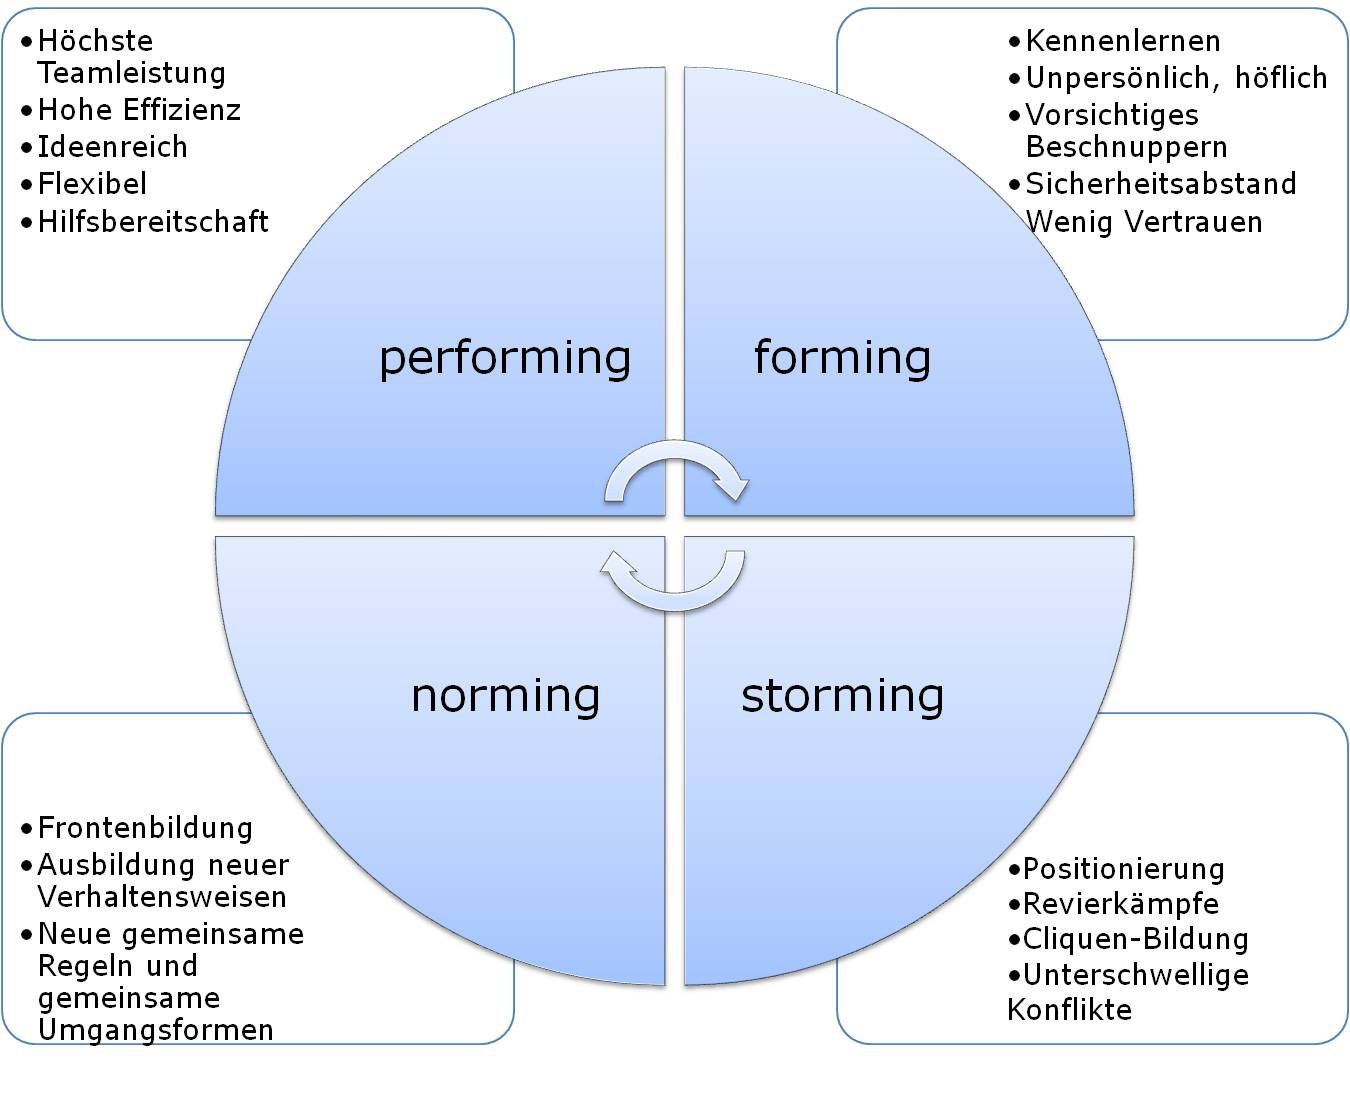
\includegraphics[width=0.7\textwidth]{Examples/Teamentwicklung.jpg}
  \caption{Die fünf Phasen der Teamentwicklung nach Tuckman}
  \label{fig:Tuckman}
\end{figure}

\chapter{Nutzen und Erkenntnisse für Softwareentwicklungs-Teams}
Ein von Hackman definiertes Autoritätsniveau ist die Fähigkeit von Teams, sich selbst zu managen. Dieses Prinzip des Selbstmanagements bedeutet, dass die Teammitglieder nicht nur für die Erledigung ihrer Aufgaben zuständig sind, sondern auch für das Management ihres Fortschritts. In vielen Kanban-Teams findet man heute dieses Prinzip, bei dem die Teammitglieder eigenständig arbeiten und ihren Fortschritt überwachen \cite{RolandWanner}.\\\\
Neben dem Selbstmanagement gibt es ein weiteres wichtiges Autoritätsprinzip in der agilen Welt: das \textit{selbstdesignende Team}. Dieses Prinzip erlaubt es den Teammitgliedern, die Struktur ihres Teams oder bestimmte Aspekte des organisatorischen Kontexts, in dem das Team arbeitet, zu verändern. Viele echte Teams und besonders Scrum-Teams, insbesondere wenn Lean/Agile skaliert wird, sind von dieser Position betroffen.\\\\
Die Möglichkeit, dass sich das Team selbst organisieren kann, führt oft zu einer Verbesserung ihrer Produktivität. Beispielsweise wissen Teammitglieder, die seit drei Monaten zusammenarbeiten, genau um die Fähigkeiten jedes einzelnen Mitglieds und können Aufgaben dementsprechend gut verteilen. Dies reduziert die Zeit für die Erledigung von Kundenprojekten und fördert ein Klima des Vertrauens mit externen Partnern.\\\\
Ein weiteres Prinzip, auf das Hackman großen Wert legt, ist das Vorhandensein eines guten Informationssystems innerhalb der Organisation. Solche Systeme helfen dem Team, ihre Leistung zu optimieren und sich an ständig ändernde Situationen anzupassen. Heute gibt es viele agile Projektmanagement-Softwares, die die Performance eines Teams messen und wichtige Leistungsindikatoren liefern können. Dazu gehören Indikatoren wie die Effektivität der Teammitglieder, der Anteil der bisher erledigten Projekte im Gesamtprojektumfang und weitere wichtige Kennzahlen.\\\\
Diese Indikatoren ermöglichen es den Teammitgliedern, ihre Projekte gut zu planen und die Produkt-Deadlines einzuhalten. Ein gutes Informationssystem unterstützt die Teams dabei, ihre Leistung kontinuierlich zu verbessern und sich flexibel an neue Herausforderungen anzupassen, was in der dynamischen und schnelllebigen Welt des agilen Projektmanagements von entscheidender Bedeutung ist.\\\\
Zusammenfassend lässt sich sagen, dass die Prinzipien des Selbstmanagements und des Selbstdesigns in agilen Teams zu einer erheblichen Steigerung der Produktivität und Effizienz führen können. Durch ein starkes Informationssystem können Teams ihre Performance überwachen und kontinuierlich verbessern, was zu einer erfolgreichen und nachhaltigen Projektumsetzung beiträgt.
\chapter*{Fazit}
Die vorliegende Arbeit hat gezeigt, dass erfolgreiches Teammanagement auf einigen zentralen Prinzipien basiert. Hackmans Konzept des Selbstmanagements ist hierbei von besonderer Bedeutung. Teams, die ihre Aufgaben und Fortschritte eigenständig überwachen und steuern, arbeiten effizienter und produktiver \cite{Hackman}. Ein weiteres wichtiges Prinzip ist das der selbstgestaltenden Teams. Diese Teams können ihre Struktur und den organisatorischen Kontext anpassen, was ihre Anpassungsfähigkeit und Effektivität erhöht. Außerdem ist ein solides Informationssystem in der Organisation unerlässlich. Solche Systeme unterstützen die Teams dabei, ihre Leistung zu optimieren und sich flexibel an Veränderungen anzupassen. Effektive Belohnungssysteme, die die Teamleistung über den individuellen Erfolg stellen, fördern die Zusammenarbeit und die Teamfähigkeit \cite{Hackman}. Schließlich ist gutes Coaching entscheidend, um die Ressourcen des Teams optimal zu nutzen und Prozessverluste zu minimieren \cite{nuernbergerCoaching}.\\\\ 
Für die Praxis ergeben sich aus diesen Erkenntnissen mehrere Empfehlungen. Unternehmen sollten Strukturen schaffen, die es den Teams ermöglichen, selbstständig zu arbeiten und ihren Fortschritt zu überwachen. Dies fördert die Eigenverantwortung und Effizienz. Der Einsatz robuster Informationssysteme ist essenziell, um die Leistung der Teams zu messen und wichtige Leistungsindikatoren bereitzustellen \cite{Hackman}. Belohnungssysteme sollten so gestaltet sein, dass sie die kollektive Leistung des Teams fördern und den Beitrag jedes einzelnen Mitglieds wertschätzen \cite{Hackman}. Coaching sollte sich an den spezifischen Bedürfnissen der Teams orientieren und Unterstützung in den jeweiligen Entwicklungsphasen bieten \cite{Hackman}. Weiterführende Fragen könnten sich auf die langfristigen Auswirkungen von Selbstmanagement und Selbstdesign auf die Teamleistung sowie auf die Evaluation unterschiedlicher Belohnungssysteme in verschiedenen organisatorischen Kontexten richten \cite{Hackman}.\\\\
Im Bereich des Teammanagements zeichnen sich einige spannende Trends ab. Die Flexibilisierung und Dezentralisierung von Teams nimmt weiter zu. Digitalisierung, KI und Big Data eröffnen neue Möglichkeiten, die Teamleistung zu überwachen und zu verbessern. Insbesondere das Management von virtuellen und hybriden Teams wird immer wichtiger, da Remote-Arbeit und hybride Arbeitsmodelle zunehmend an Bedeutung gewinnen. Digitale Kollaborationsplattformen und Kommunikations-Tools spielen hierbei eine entscheidende Rolle. Organisationen müssen zunehmend adaptiv werden und kontinuierliches Lernen fördern, um in einem sich schnell wandelnden Umfeld bestehen zu können. Diese Entwicklungen bieten nicht nur Herausforderungen, sondern auch zahlreiche Möglichkeiten, die Effektivität und Effizienz von Teams weiter zu steigern. Es bleibt spannend zu beobachten, wie diese Trends in der Praxis umgesetzt werden und welche neuen Ansätze sich in der Zukunft als besonders wirkungsvoll erweisen.

